\documentclass{article}

\usepackage[preprint]{neurips_2026}

\usepackage[utf8]{inputenc}
\usepackage[T1]{fontenc}
\usepackage{hyperref}
\usepackage{url}
\usepackage{booktabs}
\usepackage{amsfonts}
\usepackage{amsmath}
\usepackage{nicefrac}
\usepackage{microtype}
\usepackage{xcolor}
\usepackage{graphicx}
\usepackage{float}

\title{The Language of Electoral Competition:\\Thematic Structure and Ideological Framing\\in French Legislative Manifestos, 1973--1993}

\author{
  Gabriel Orsatti\thanks{Course: Machine Learning for Natural Language Processing.} \\
  ENSAE Paris -- Institut Polytechnique de Paris\\
  M2 Data Science, 2025--2026\\
  \texttt{gabriel.orsatti@ensae.fr}
}

\begin{document}

\maketitle

\begin{abstract}
This paper applies natural language processing to 21,697 French electoral manifestos (\textit{professions de foi}) from five legislative elections between 1973 and 1993. We combine LDA topic modeling, logistic regression on TF-IDF, and log-odds rhetorical analysis to ask two questions: what thematic structure organises political discourse, and how do political families frame shared policy themes differently? An 11-topic LDA model produces a balanced thematic decomposition covering class struggle, ecology, immigration, social protection, and governance. A logistic regression classifier predicts political family from text alone with strong accuracy, and the log-odds analysis reveals that families discussing the same topic---say, unemployment---use strikingly different vocabularies. We also compare discourse to INSEE macroeconomic data and find that campaign rhetoric partly tracks material conditions. The main insight: ideological differentiation operates at the vocabulary level, not the topic level. All families discuss the same broad themes; they just talk about them differently.
\end{abstract}

\section{Introduction}

In France, the \textit{profession de foi} is a short electoral manifesto printed at public expense and mailed to every registered voter before each round of legislative voting. The document is simultaneously official and partisan, constrained in format but free in content---one of the few standardised records of what parties choose to say to voters at a given moment.

The Archelec corpus, digitised by Sciences Po Paris and the CEVIPOF, gathers these manifestos from 1958 to 1993, with OCR transcriptions by the Teklia laboratory. We focus on five legislative elections---1973, 1978, 1981, 1988, and 1993---spanning the end of the Gaullist era, the \textit{alternance} of 1981, the rise of the Front National, and the emergence of political ecology. Our question: can we recover the ideological structure of the French party system from text alone?

We proceed in three stages. First, unsupervised topic models identify latent themes (Section~\ref{sec:topics}). Second, supervised classification tests whether text predicts political family (Section~\ref{sec:classification}). Third, log-odds ratios and macroeconomic data reveal how families frame shared themes differently (Section~\ref{sec:framing}).

\section{Related work}

The Comparative Manifesto Project \citep{budge2001mapping} pioneered cross-national manifesto coding, but manual annotation is expensive. Automated methods \citep{grimmer2013text} transformed the field: bag-of-words and TF-IDF proved effective because political vocabulary is highly repetitive. LDA \citep{blei2003latent} became the dominant unsupervised method, applied to U.S. Senate speeches \citep{quinn2010analyze} and extended with metadata \citep{roberts2014structural}. For French political corpora, lexicometric approaches \citep{bonnafous2003analyse} exist but not at the scale of the full Archelec collection.

The ``fighting words'' framework \citep{monroe2008fightin} identifies vocabulary disproportionately favoured by one group, controlling for verbosity via an informative Dirichlet prior. NMF \citep{lee1999learning} and BERTopic \citep{grootendorst2022bertopic} offer alternatives to LDA; we experiment with all three. On the supervised side, logistic regression on TF-IDF remains a strong interpretable baseline \citep{joachims1998text}.

\section{Data and preprocessing}
\label{sec:data}

The corpus combines metadata from the Archelec catalogue (33,031 entries, 42 columns) with OCR transcriptions from ZIP archives. After joining on document identifiers (97.6\% match rate), the working dataset contains 21,697 manifestos across the five elections.

\textbf{Preprocessing.} Lowercasing, punctuation/digit removal, tokenization, three-layer stopword filtering (function words, domain terms, OCR watermarks), and lemmatisation via spaCy. Short documents ($<$100 characters) and German-language manifestos from Alsace-Moselle are excluded.

\textbf{Political families.} Raw party labels (hundreds of unique strings) are aggregated into six families: \textit{Gauche radicale} (PCF, LO, LCR), \textit{Gauche modérée} (PS, MRG), \textit{Écologistes}, \textit{Centre} (UDF, CDS), \textit{Droite} (RPR), and \textit{Extrême droite} (FN). Unaffiliated documents (18.6\%) are excluded.

\textbf{Profession mapping.} The 2,000+ unique profession strings are classified into 15 PCS categories via zero-shot NLI with XLM-RoBERTa \citep{conneau2020unsupervised}.

\section{Exploratory analysis}
\label{sec:exploration}

\begin{figure}[H]
\centering
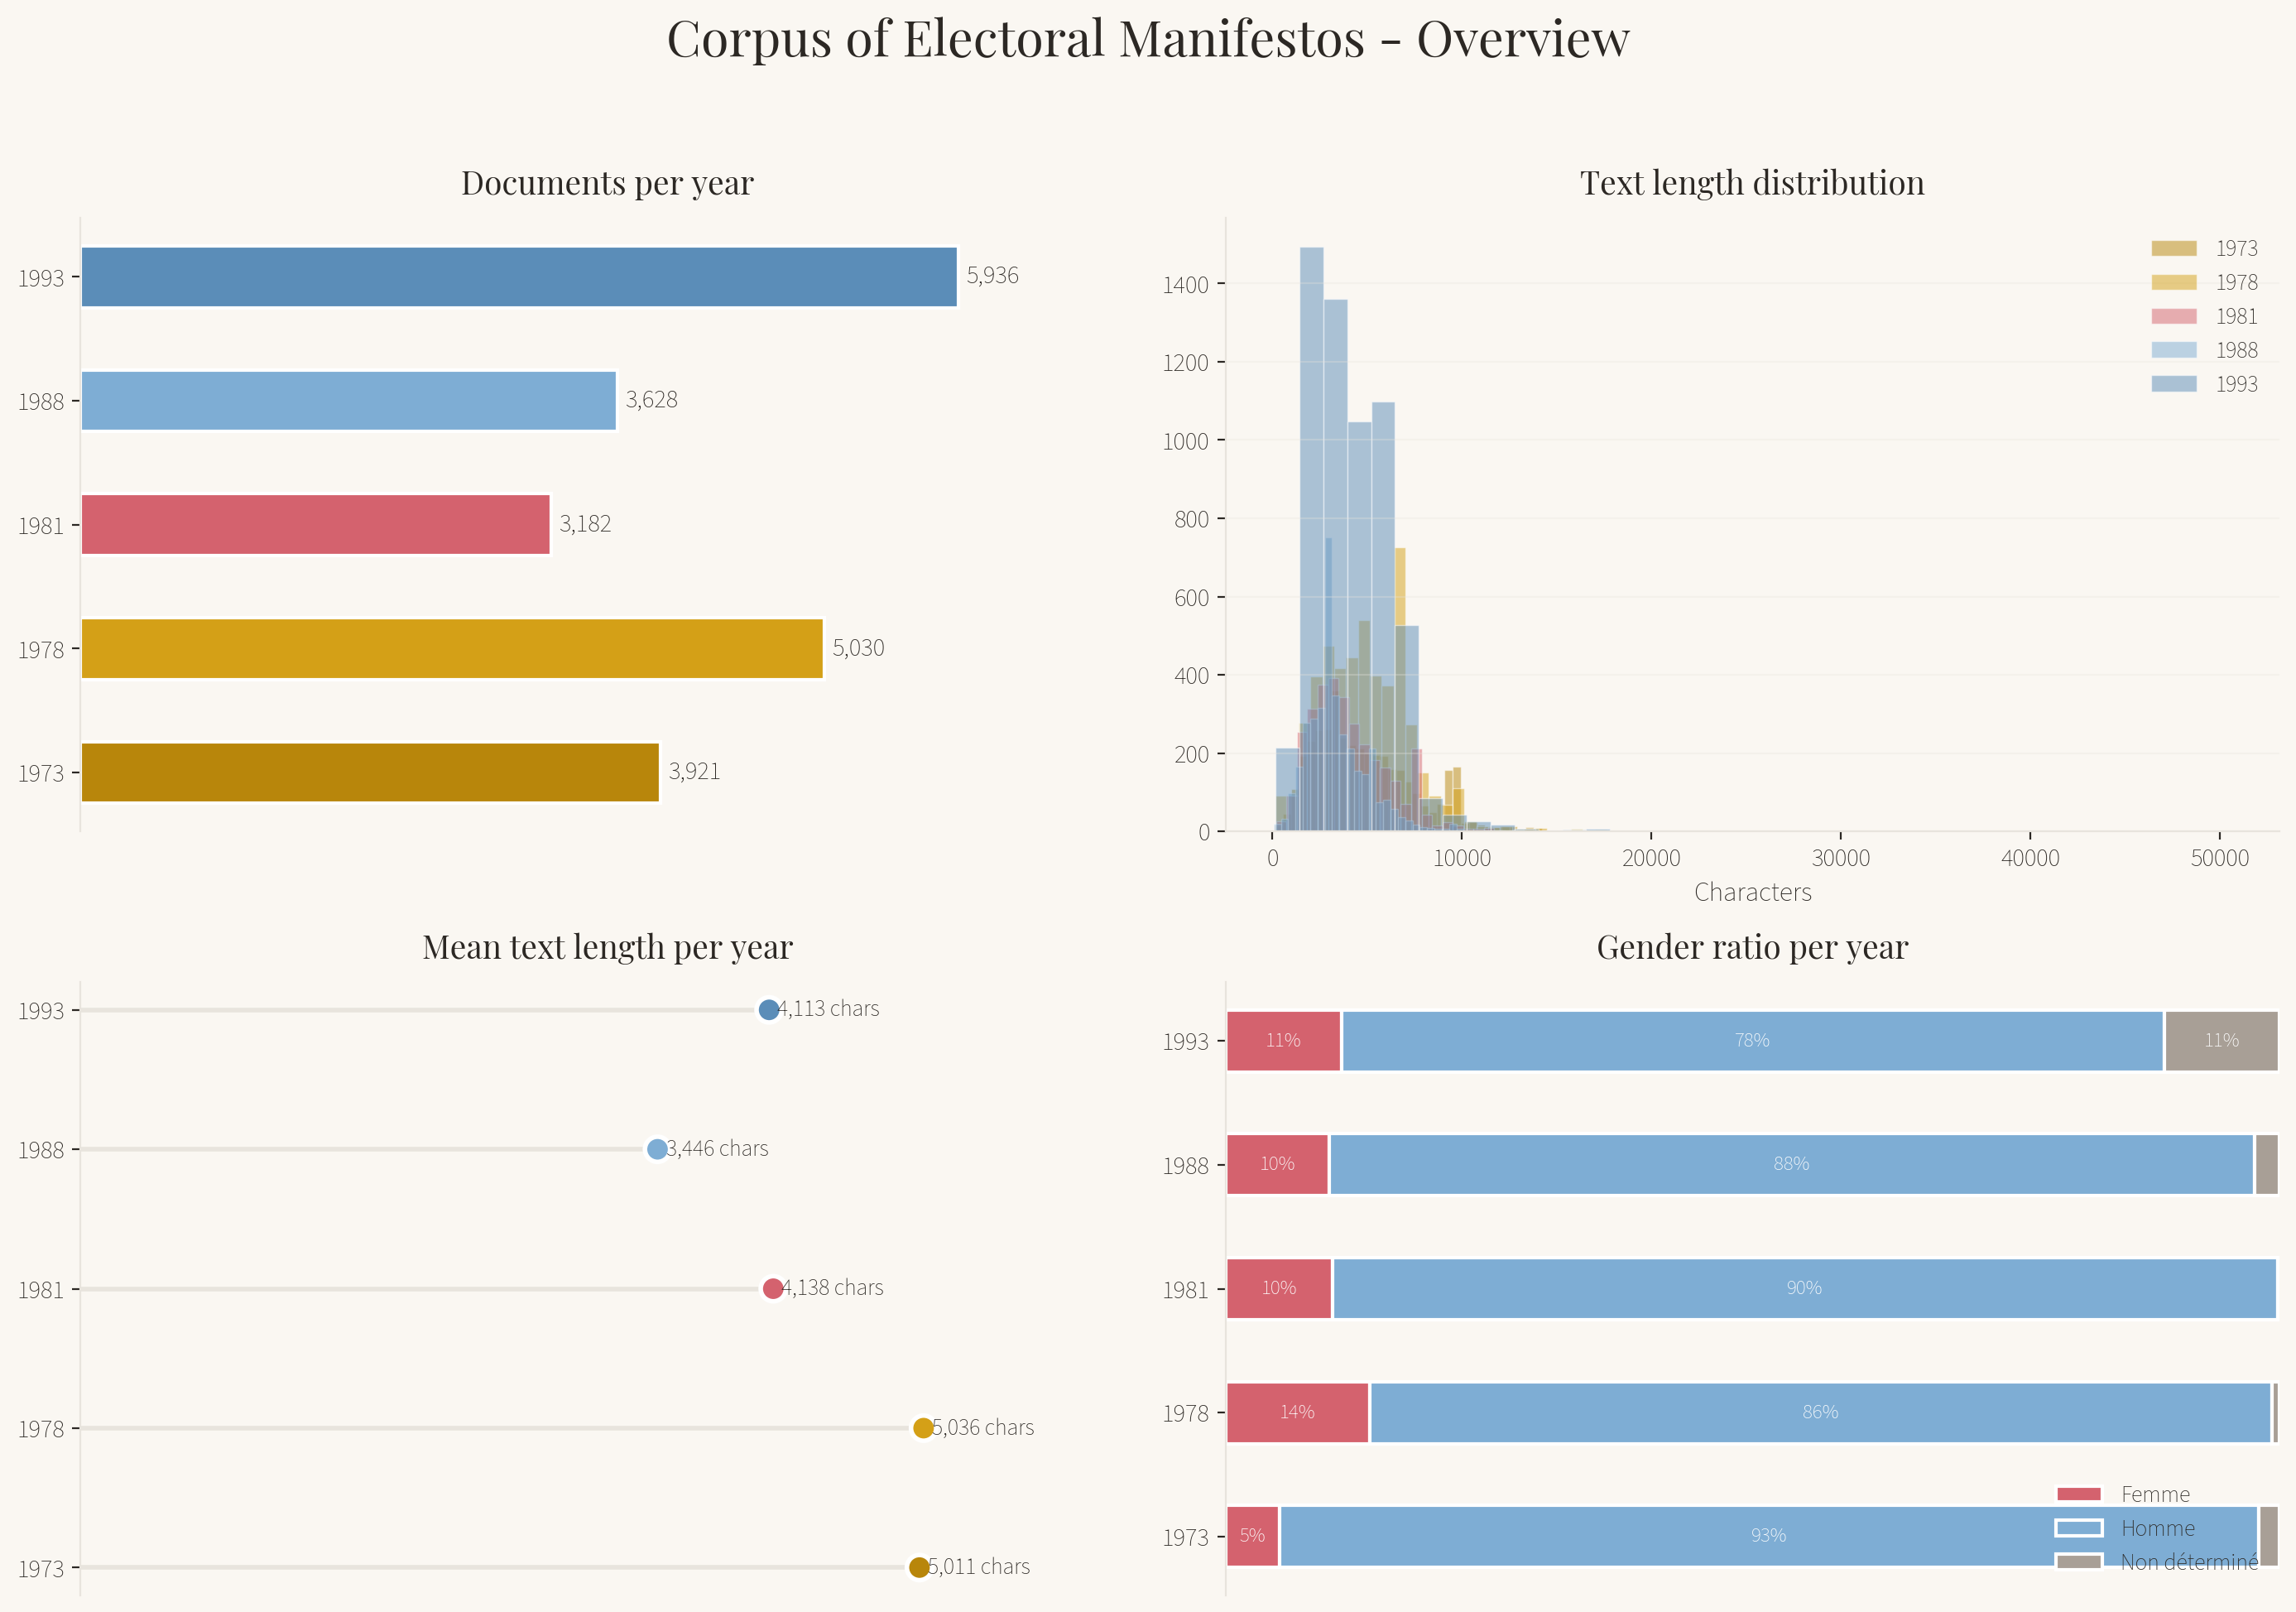
\includegraphics[width=\linewidth]{exploration_base.png}
\caption{Corpus overview: documents per year, text-length distribution, mean text length, and gender ratio. Candidacies grow from 3,900 (1973) to 6,000 (1993); 82\%+ of candidates are male throughout.}
\label{fig:exploration}
\end{figure}

Figure~\ref{fig:exploration} summarises the corpus. Candidacy growth reflects party-system fragmentation; text length stays consistent (3,400--5,000 characters), constrained by the physical leaflet format.

\begin{figure}[H]
\centering
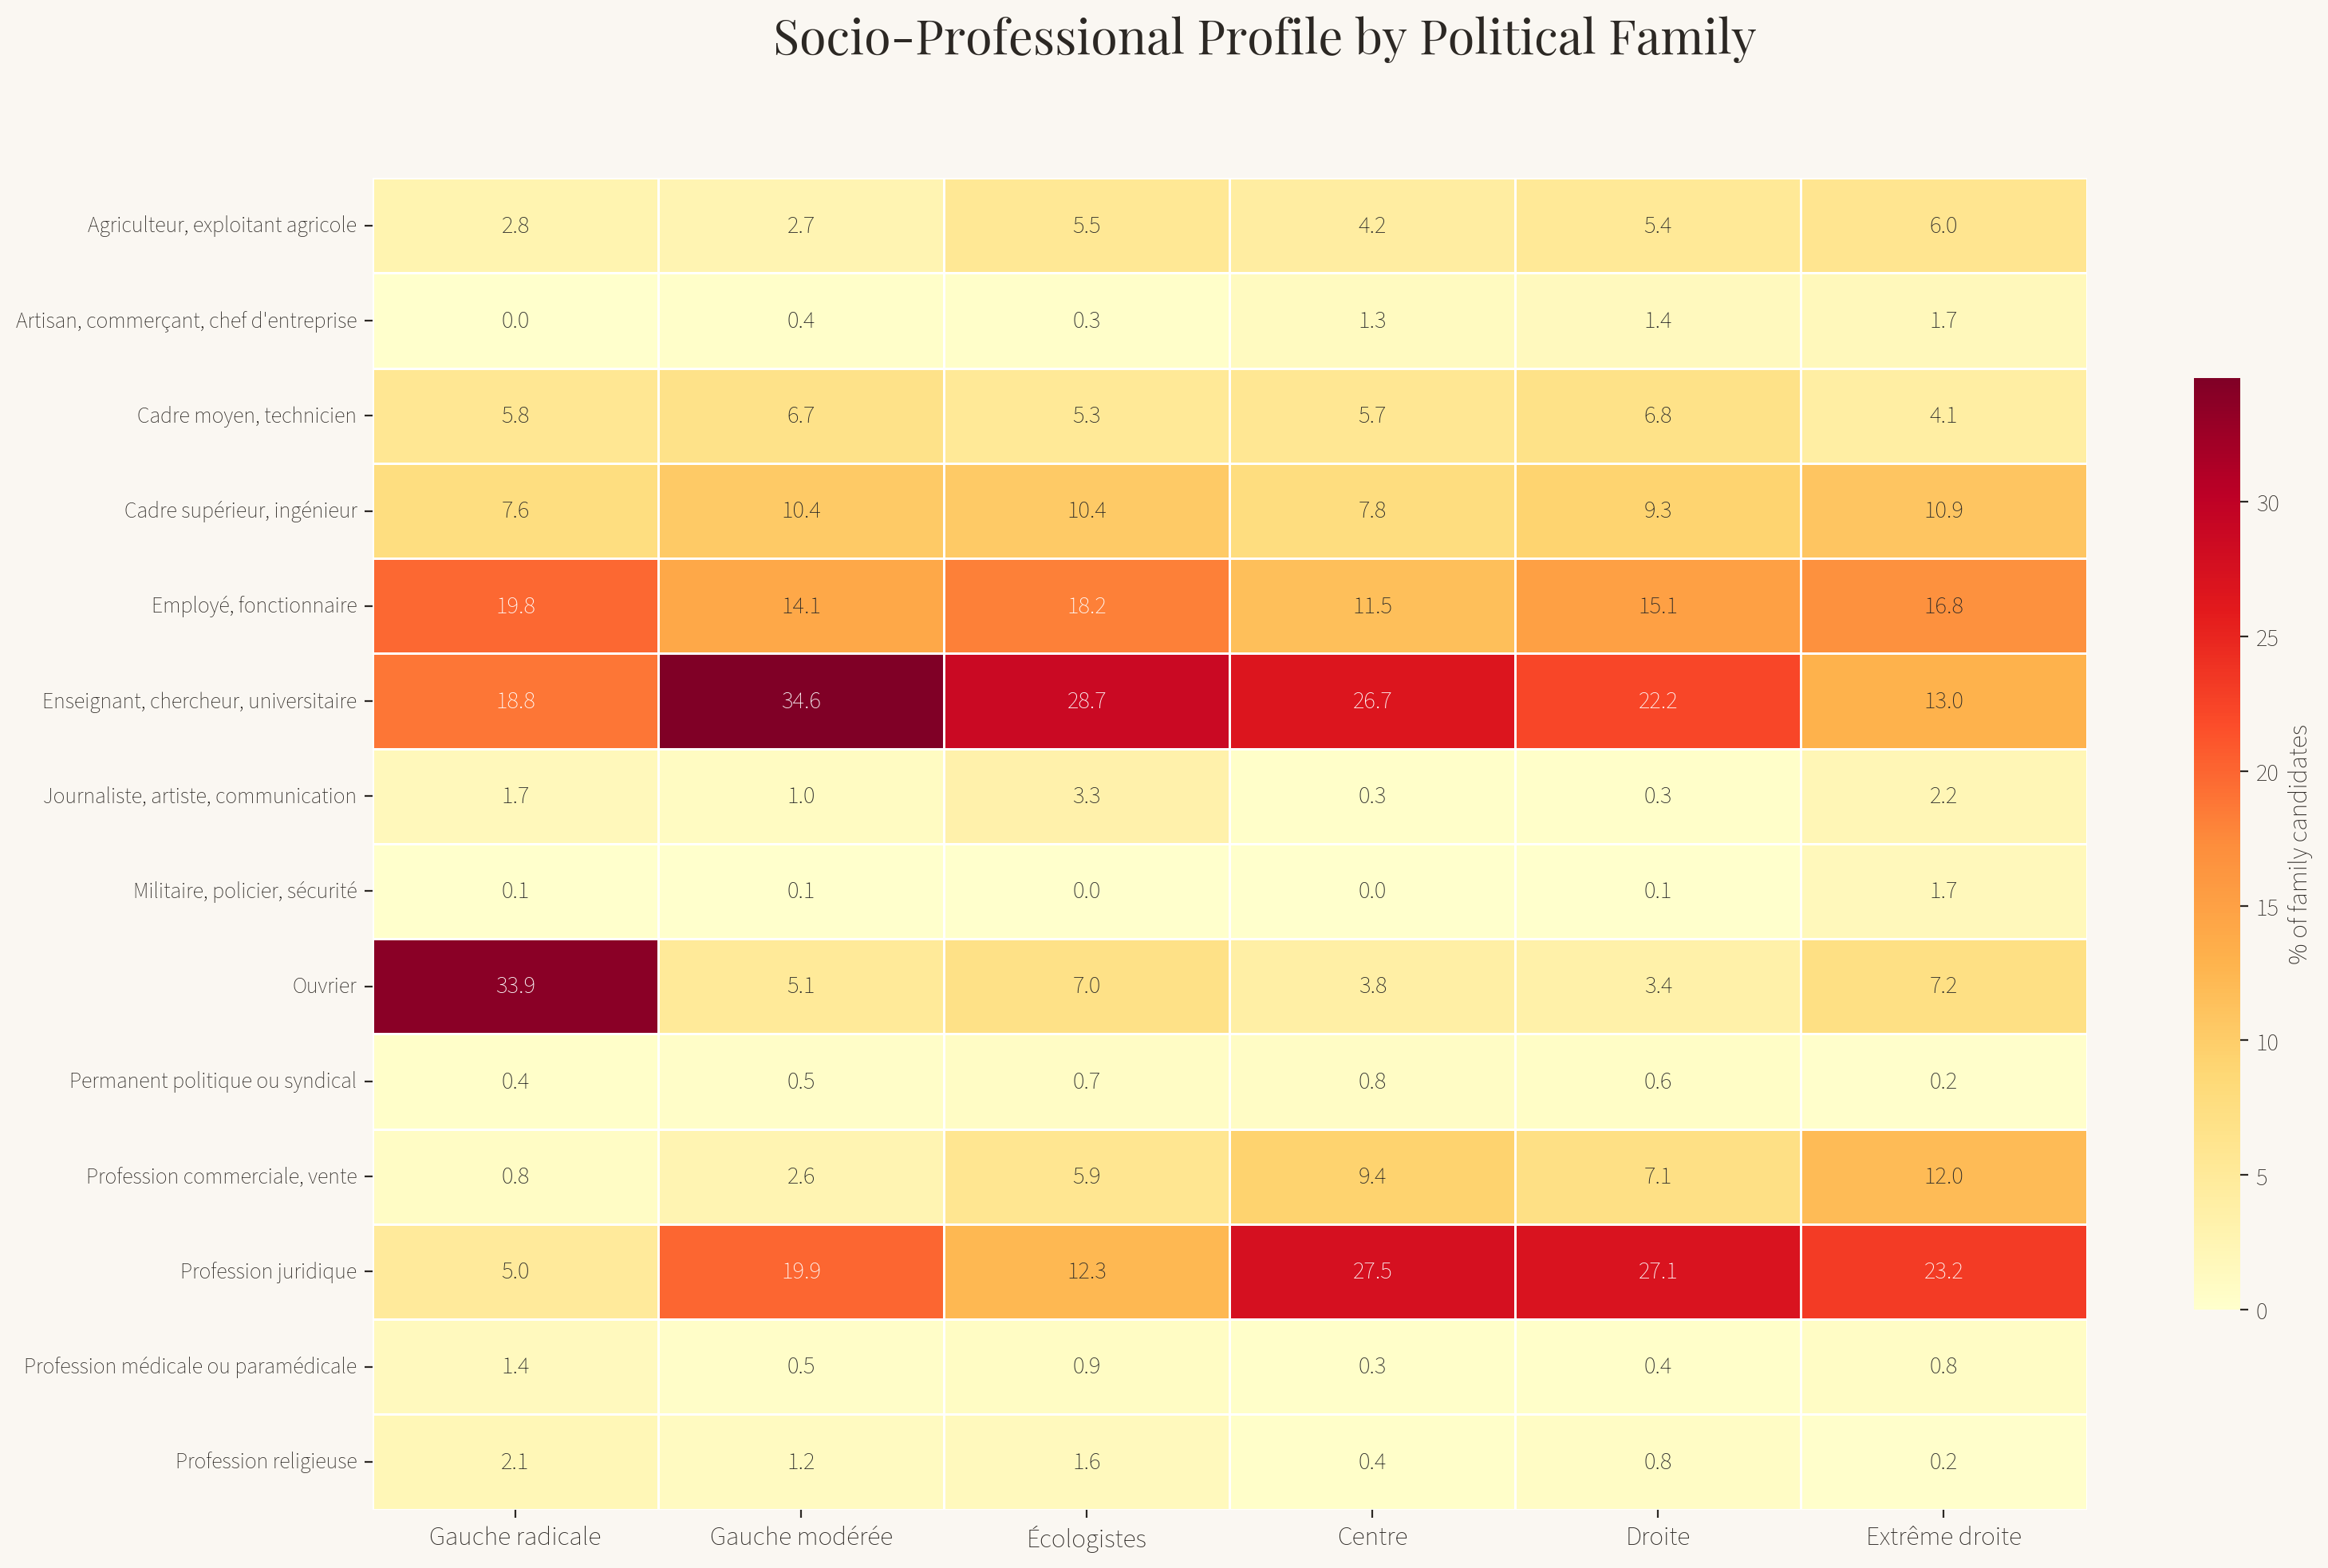
\includegraphics[width=0.85\linewidth]{heatmap_pcs_partis.png}
\caption{Cross-tabulation of BERT-classified PCS categories and political families. Teachers dominate the \textit{Gauche modérée}; blue-collar workers the \textit{Gauche radicale}; executives and lawyers the \textit{Droite}/\textit{Centre}.}
\label{fig:pcs}
\end{figure}

The PCS heatmap (Figure~\ref{fig:pcs}) reveals the sociological bases of each tradition, consistent with the political sociology literature \citep{gaxie1978cens}. These well-documented patterns validate our zero-shot classification pipeline.

\section{Topic modeling}
\label{sec:topics}

\subsection{Model selection}

We train LDA on raw counts (unigrams/bigrams, 10,000 terms) and NMF on TF-IDF (3,000 terms). Optimal $k$ is selected by $C_v$ coherence \citep{roder2015exploring}, with a balance constraint: models where the largest topic exceeds 50\% are rejected. A critical preliminary step is removing $\sim$200 partisan terms (party names, leaders, slogans) identified through a baseline diagnostic; without this, both models latch onto party identity rather than policy content.

\begin{figure}[H]
\centering
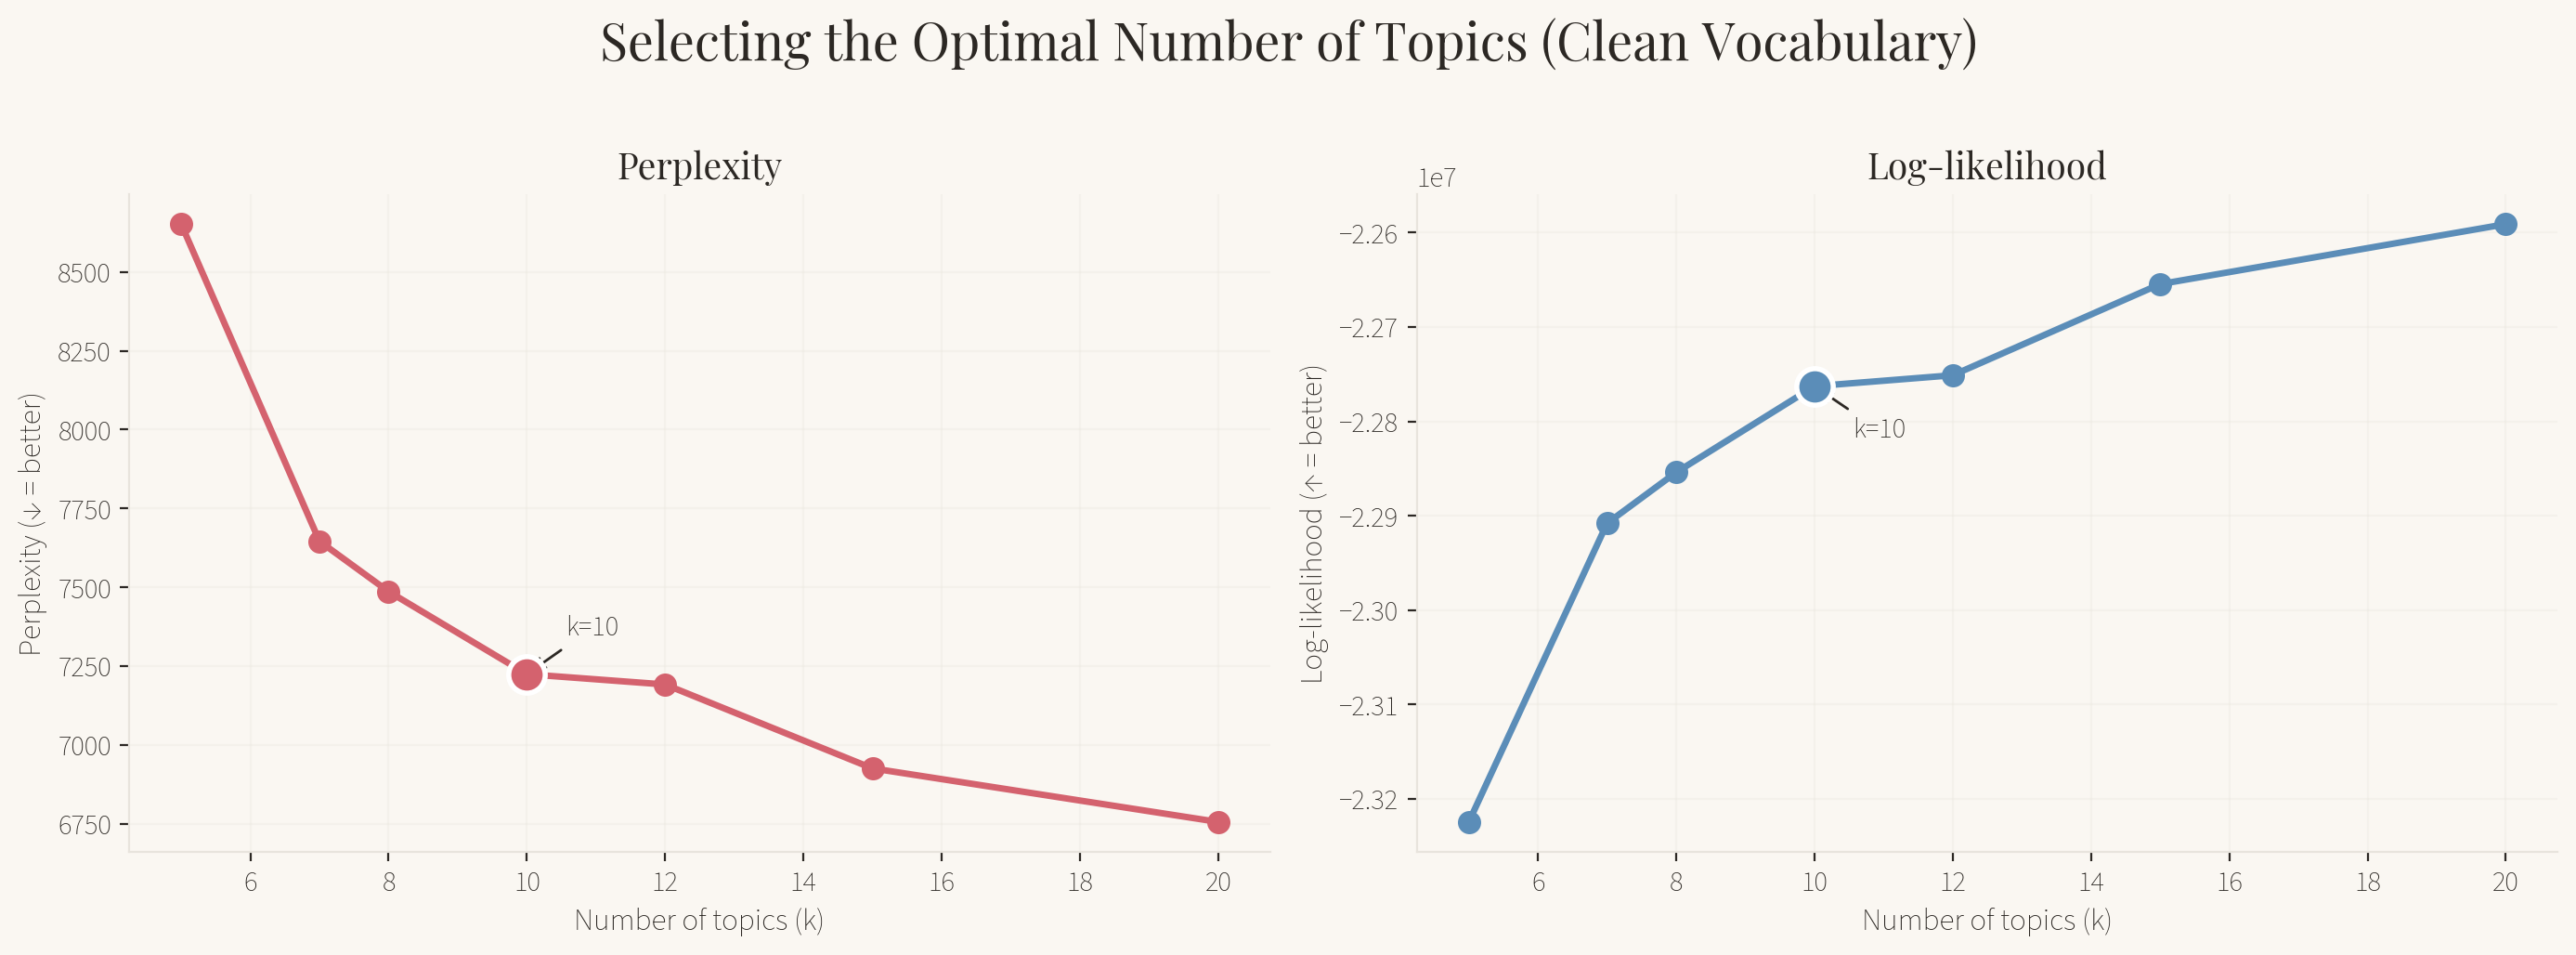
\includegraphics[width=0.75\linewidth]{optimal_k_clean.png}
\caption{$C_v$ coherence vs.\ number of topics. LDA peaks at $k{=}11$ with balanced distribution (no topic $>$24\%). NMF peaks at $k{=}5$ but concentrates 84.5\% of documents in one topic---analytically useless.}
\label{fig:coherence}
\end{figure}

After grid search (Figure~\ref{fig:coherence}), LDA at $k{=}11$ achieves $C_v = 0.49$ with no topic exceeding 24\% of the corpus. NMF at $k{=}5$ scores $C_v = 0.71$ but is degenerate. We select LDA.

\subsection{Topic structure}

\begin{figure}[H]
\centering

\includegraphics[width=\linewidth]{lda_topic_words.png}
\caption{Top words per LDA topic (partisan vocabulary removed). Three clusters emerge: labour and class struggle (Topics 0, 5, 9), institutional governance (1, 3, 4), and issue-specific themes---ecology (2, 7, 10), immigration (8), social protection (6).}
\label{fig:topics}
\end{figure}

The 11 topics (Figure~\ref{fig:topics}) form three clusters. The \textbf{labour block} (Topics 0, 5, 9) spans employer--employee dynamics, militant Marxist vocabulary, and the 1981 Mitterrandist mobilisation. The \textbf{institutional block} (1, 3, 4) captures presidential-majority rhetoric, left-wing alliance language, and right-wing coalition discourse. \textbf{Issue topics} cover ecology (three topics tracking the movement's evolution), FN immigration rhetoric (8), and social protection (6).

\subsection{Temporal dynamics and political family specialisation}

\begin{figure}[H]
\centering

\includegraphics[width=0.9\linewidth]{party_specialization.png}
\caption{Topic specialisation by political family. Over-representation ratio ($>$1 means the family discusses the topic more than average). Niche families (radical left, far right, ecologists) show strong specialisation; mainstream families (centre, right) are more diffuse.}
\label{fig:specialisation}
\end{figure}

Figure~\ref{fig:specialisation} quantifies thematic specialisation. Niche families---\textit{Gauche radicale}, \textit{Extrême droite}, \textit{Écologistes}---show strong over-representation in their signature topics. Mainstream families (\textit{Droite}, \textit{Centre}) have flatter profiles. Yet all families share broadly similar topic distributions: the differentiation happens not in \textit{what} they discuss but in \textit{how}---motivating Section~\ref{sec:framing}.

\section{Supervised classification}
\label{sec:classification}

Given only the text, can a classifier determine which family wrote it? We train logistic regression (L2) on TF-IDF features (unigrams and bigrams, 10,000 features) with 5-fold stratified cross-validation.

\begin{figure}[H]
\centering
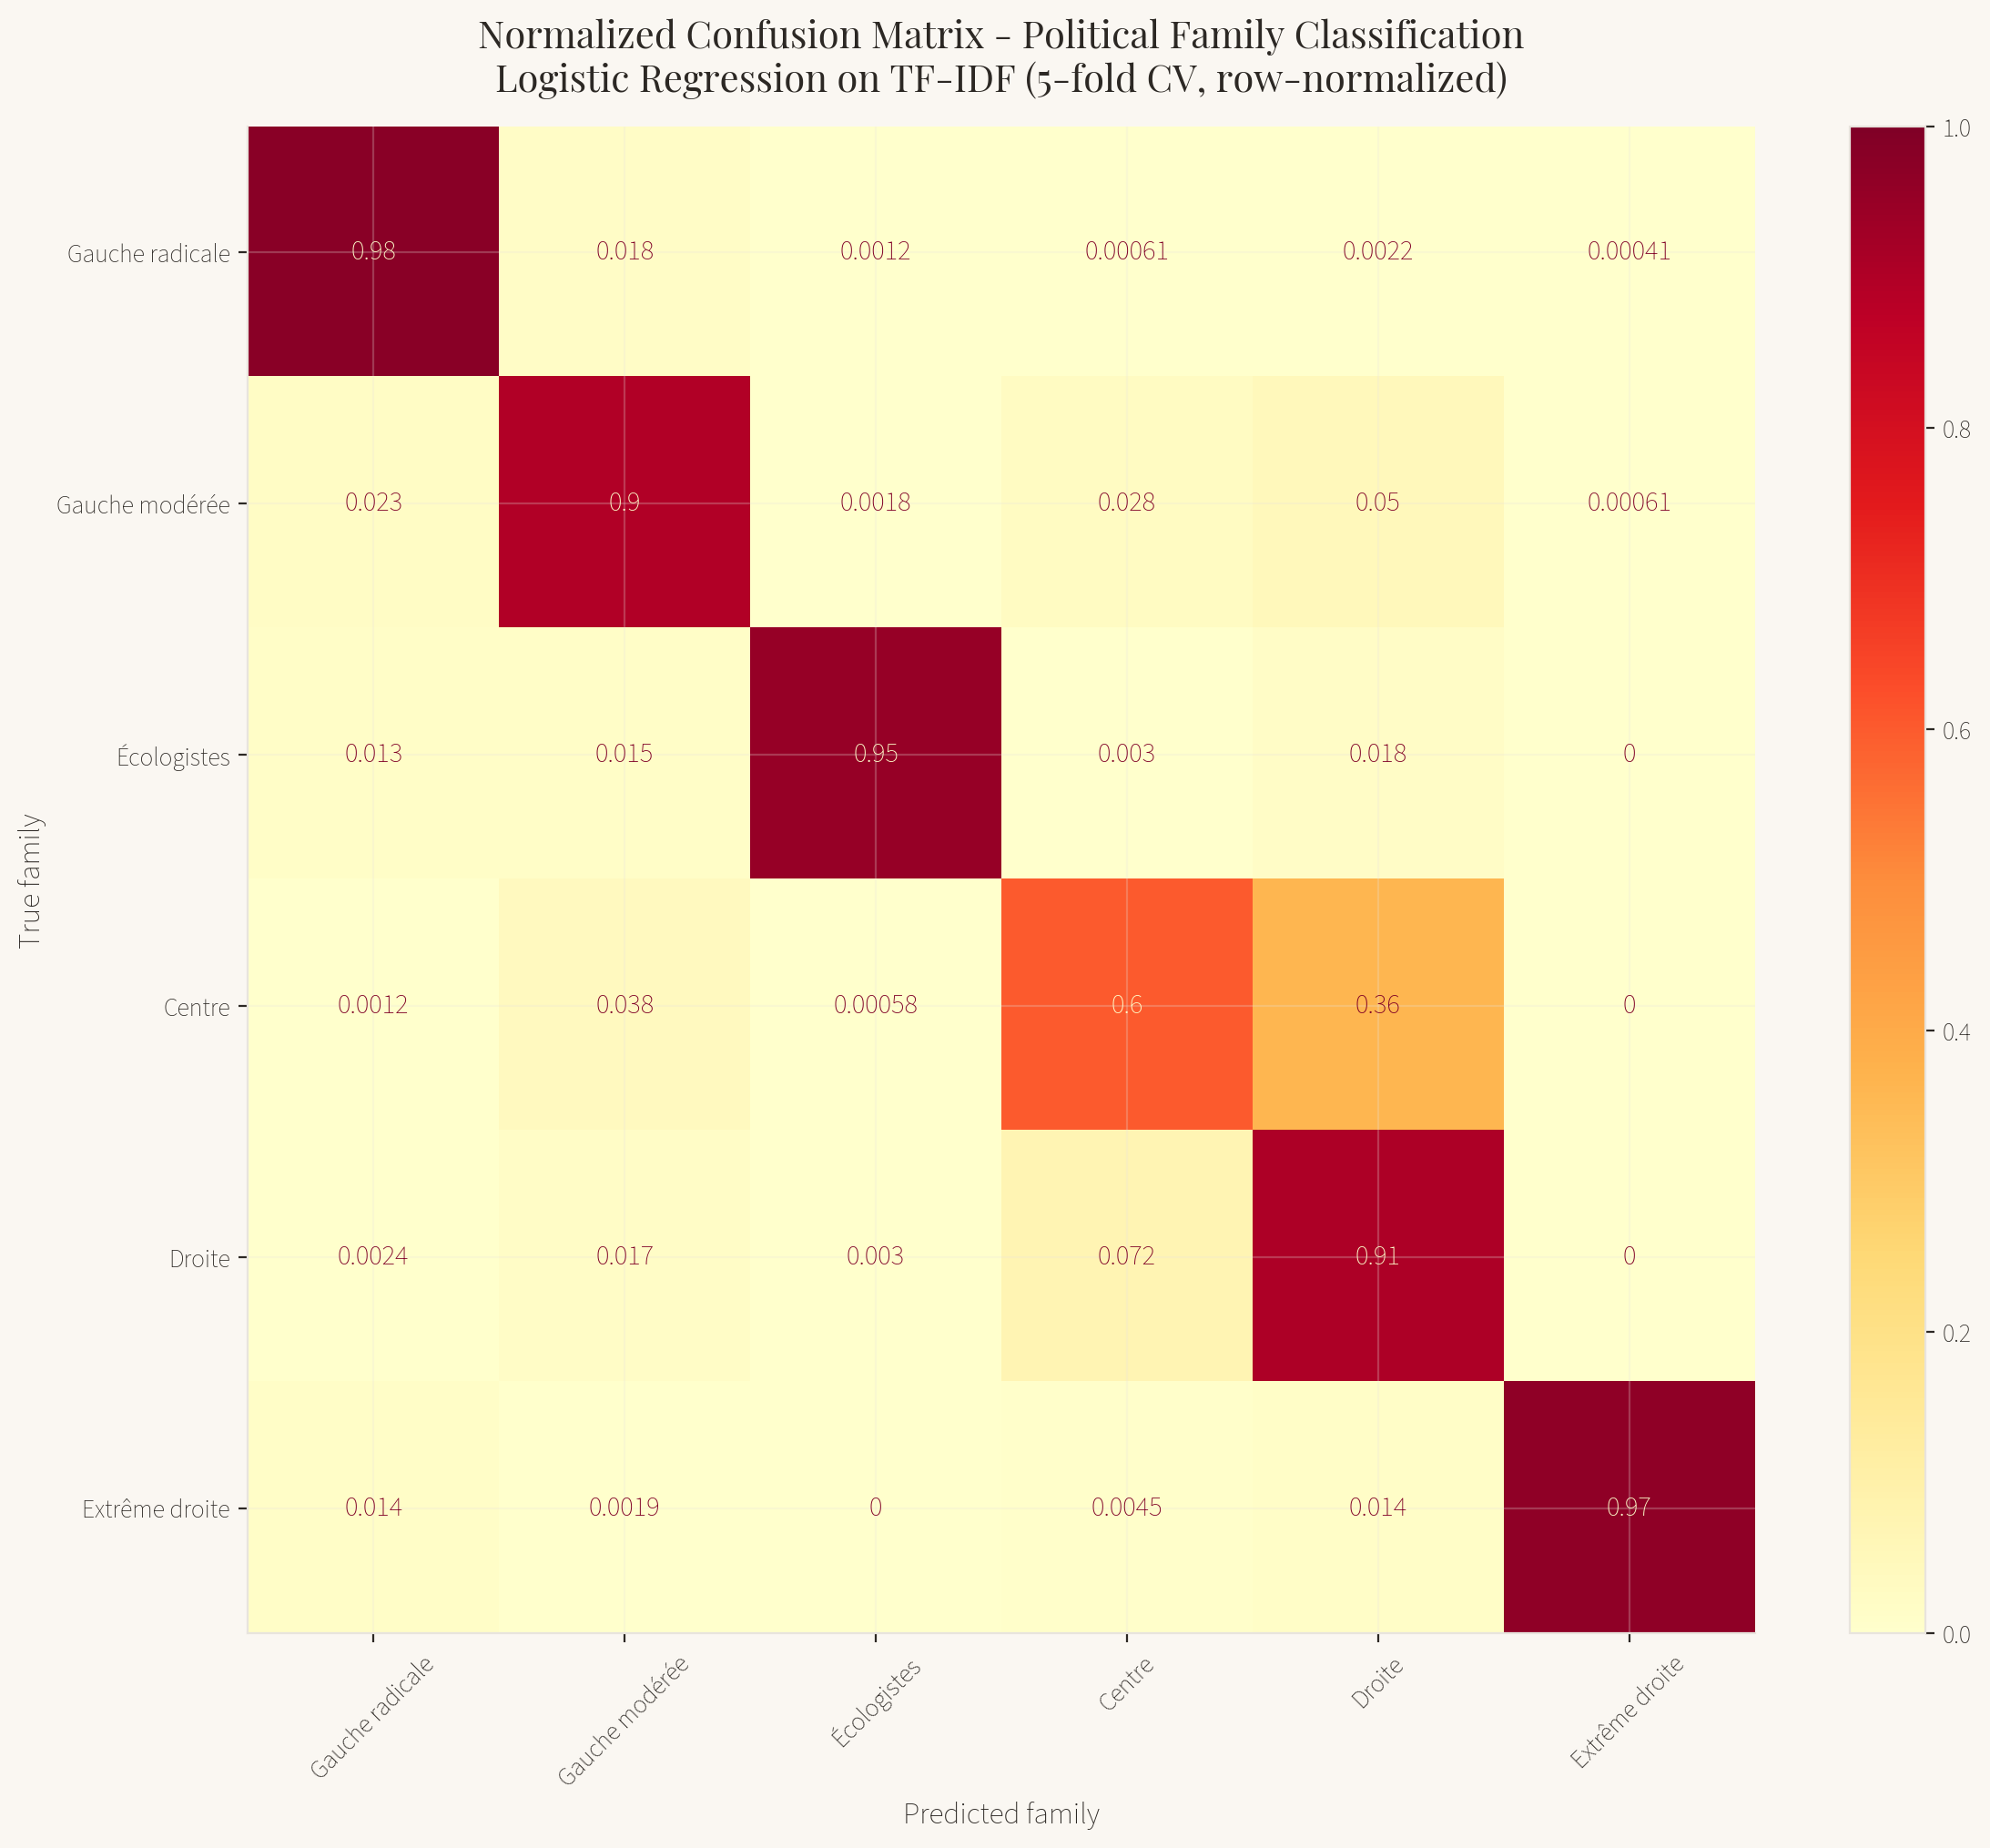
\includegraphics[width=\linewidth]{confusion_matrix.png}
\caption{Normalised confusion matrix (logistic regression, 5-fold CV). Gauche radicale and Extrême droite achieve the highest diagonal values. Centre is most confused with Droite, reflecting genuine vocabulary overlap from decades of governing together.}
\label{fig:confusion}
\end{figure}

The confusion matrix (Figure~\ref{fig:confusion}) reveals a hierarchy of classifiability: \textit{Gauche radicale} and \textit{Extrême droite} are classified accurately; \textit{Centre} is frequently confused with \textit{Droite}, reflecting genuine vocabulary overlap from decades of governing together.

\begin{figure}[H]
\centering
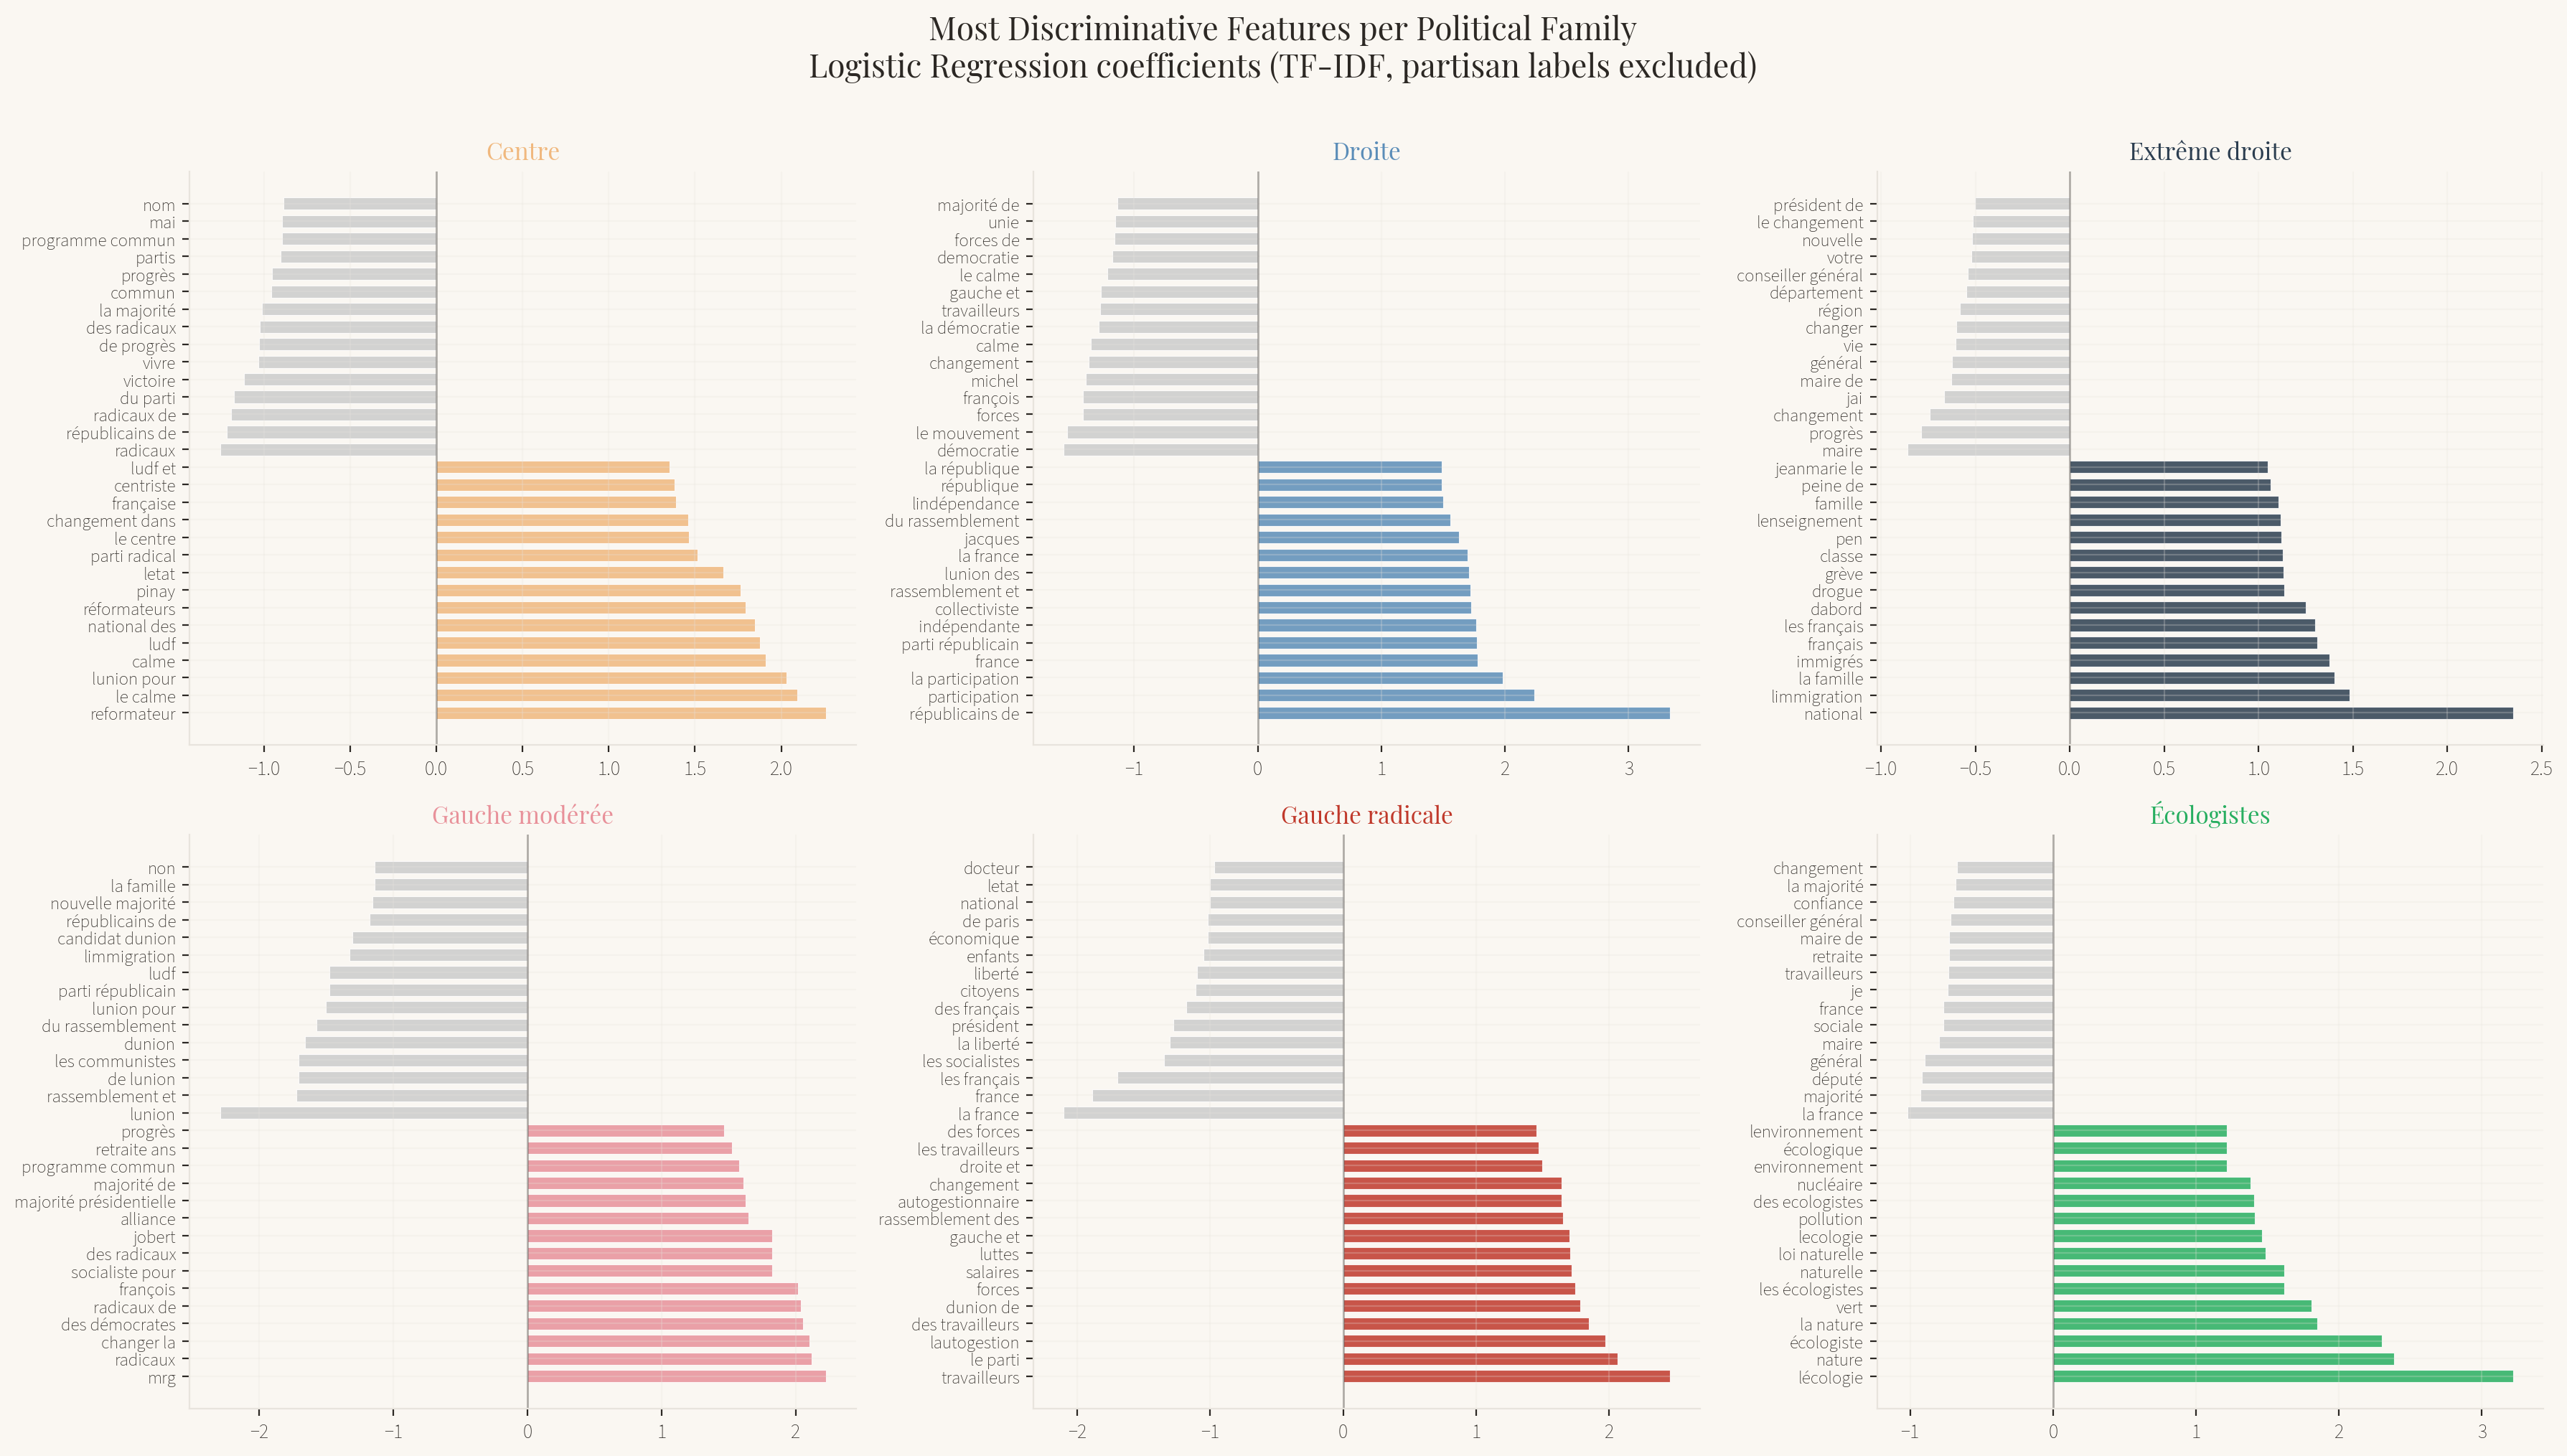
\includegraphics[width=\linewidth]{lr_features_by_family.png}
\caption{Most discriminative TF-IDF features per family (logistic regression coefficients, partisan labels filtered out). Class struggle for the radical left, immigration for the far right, ecology for the Greens, enterprise vocabulary for the right.}
\label{fig:features}
\end{figure}

After filtering party names, Figure~\ref{fig:features} exposes each family's ideological lexicon. These signatures align with topic-level specialisation but provide finer grain. The learning curve plateaus at $\sim$60\% of training data, suggesting model expressiveness---not data quantity---is the bottleneck.

\section{Rhetorical framing and macroeconomic context}
\label{sec:framing}

\subsection{Fighting words}

Topic models show \textit{that} families share themes; the question is \textit{how} they frame them. We use log-odds ratios with informative Dirichlet prior \citep{monroe2008fightin}:
\[
\delta^{(A,B)}_w \!=\! \log\!\tfrac{f^A_w + \alpha}{N^A + V\alpha} - \log\!\tfrac{f^B_w + \alpha}{N^B + V\alpha}
\]
where $f^A_w$ counts word $w$ in family $A$'s documents on topic $t$ and $\alpha$ smooths for verbosity.

\begin{figure}[H]
\centering

\includegraphics[width=\linewidth]{fighting_words_employment.png}
\caption{Fighting words on the employment topic. The radical left frames unemployment through \textit{travailleurs} and \textit{patronat}; the far right through \textit{immigration} and \textit{insécurité}; the moderate left uses \textit{emploi}, \textit{formation}; the right invokes \textit{entreprise} and \textit{charges}. Same topic, different worlds.}
\label{fig:fighting}
\end{figure}

Figure~\ref{fig:fighting} shows the employment topic. The radical left speaks of \textit{travailleurs}, \textit{patronat}---class conflict. The far right frames the same reality through \textit{immigration} and \textit{insécurité}. The moderate left uses a managerial register (\textit{emploi}, \textit{formation}). The right invokes \textit{entreprise} and \textit{charges}. Same policy domain, radically different rhetorical universes.

\subsection{Discourse vs.\ macroeconomic reality}

\begin{figure}[H]
\centering
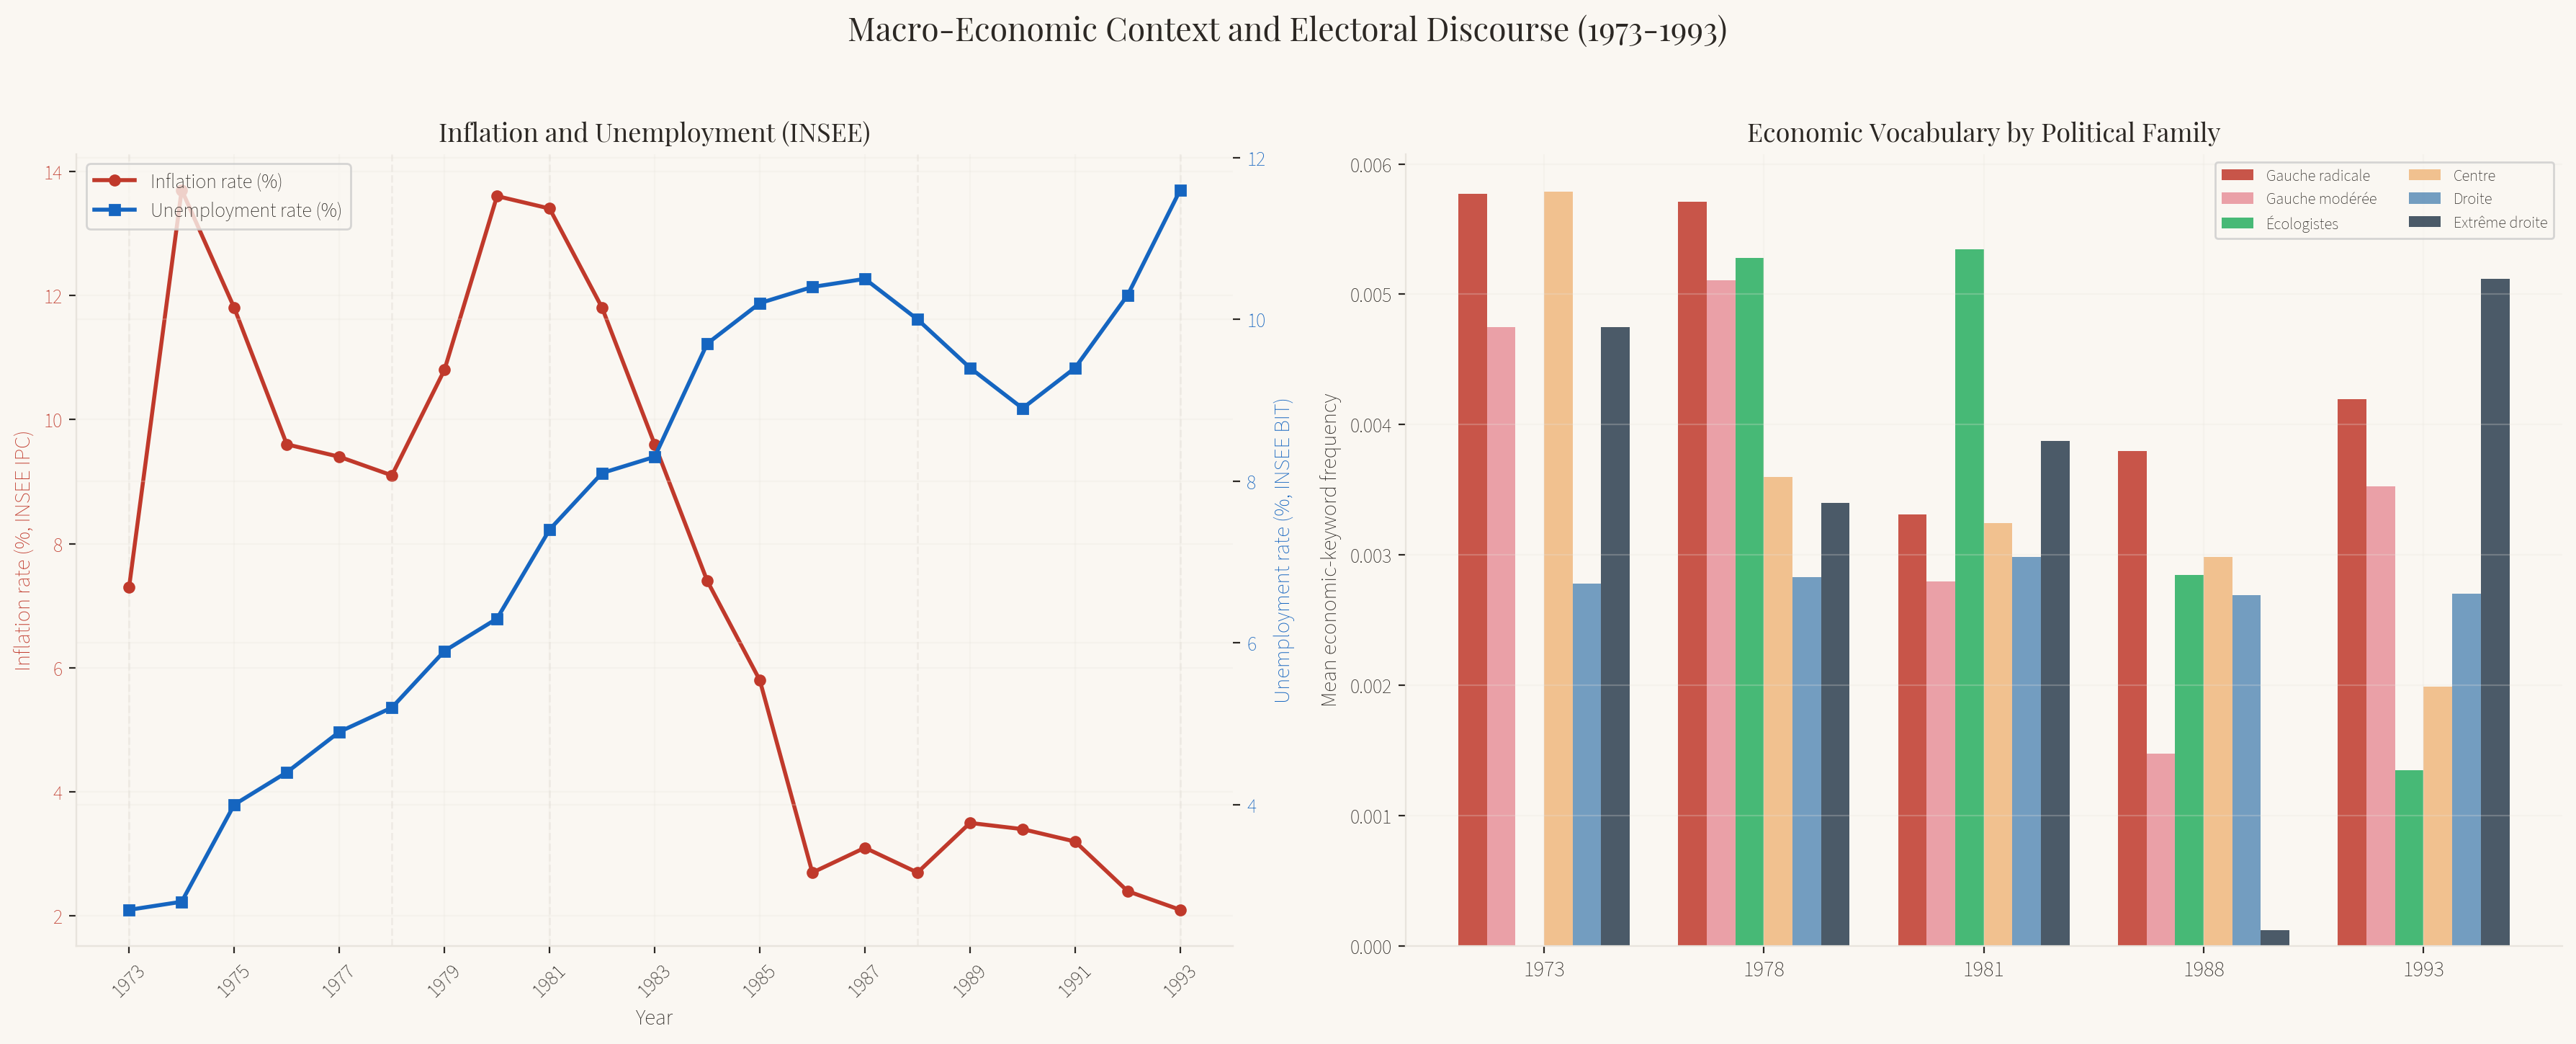
\includegraphics[width=\linewidth]{macro_econ_extended.png}
\caption{Left: national inflation and unemployment (INSEE). Right: economic vocabulary frequency in manifestos by family. Discourse broadly tracks macroeconomic stress---highest in 1978--1981 (stagflation), declining in 1988 (disinflation), rebounding in 1993 (recession).}
\label{fig:macro}
\end{figure}

Figure~\ref{fig:macro} overlays INSEE data with economic vocabulary frequency. Economic vocabulary peaks in 1978--1981 (stagflation era, inflation at 13.4\%), declines in 1988 as inflation recedes, then rebounds in 1993---now oriented toward unemployment (11.6\%) rather than prices. Campaign rhetoric is partly responsive to material conditions, not purely strategic.

\section{Semantic geometry}

\begin{figure}[H]
\centering

\includegraphics[width=0.85\linewidth]{tsne_by_family.png}
\caption{t-SNE projection of LDA topic vectors ($n{=}21{,}139$, perplexity${}=50$, cosine distance). Gauche radicale and Extrême droite occupy isolated regions; Droite and Centre overlap considerably; Gauche modérée bridges the left and institutional themes.}
\label{fig:tsne}
\end{figure}

The t-SNE projection (Figure~\ref{fig:tsne}) maps 11-dimensional topic vectors to two dimensions \citep{vandermaaten2008}. \textit{Gauche radicale} and \textit{Extrême droite} form isolated clusters; \textit{Droite} and \textit{Centre} overlap heavily. The geometry confirms every other analysis: ideological extremes are distinctive, the centre is diffuse.

\section{Discussion}

Three findings deserve emphasis. First, unsupervised and supervised methods complement each other: topic modeling reveals shared themes; classification shows families are nonetheless distinguishable; fighting words show the distinction operates through vocabulary, not topics. Second, the hierarchy of classifiability is informative---niche parties cultivate distinctive discursive identities while catch-all parties blur them \citep{meguid2005competition}. Third, the temporal dimension captures genuine political dynamics: immigration discourse tracks the FN's breakthrough, class-struggle vocabulary mirrors the PCF's decline, and ecology follows the Green movement's institutionalisation.

\textbf{Limitations.} OCR quality varies (worse for 1973, 1978). Class imbalance affects minority-class reliability. We use hard topic assignments ($\arg\max$) rather than soft memberships. The discourse--reality correlation is ecological \citep{robinson1950ecological}. Transformer-based classifiers (CamemBERT) might improve harder classes.

\section{Conclusion}

Political differentiation in French electoral manifestos operates at the vocabulary level, not the topic level. All families discuss the same themes; they frame them through ideologically distinctive language. Supervised and lexical methods---logistic regression, log-odds ratios---are needed to capture this variation, which topic models alone miss. Classical NLP methods carry the analysis further than one might expect: interpretable baselines let you read the coefficients and understand \textit{why} a document belongs where it does. A natural extension is fine-tuned CamemBERT for studying how the semantics of political words shift across elections.

\medskip

{
\small

\bibliographystyle{plainnat}
\begin{thebibliography}{99}

\bibitem[Blei et~al.(2003)]{blei2003latent}
Blei, D.~M., Ng, A.~Y., and Jordan, M.~I. (2003).
Latent {D}irichlet {A}llocation.
\textit{JMLR}, 3:993--1022.

\bibitem[Bonnafous and Tournier(2003)]{bonnafous2003analyse}
Bonnafous, S. and Tournier, M. (2003).
Analyse du discours, lexicométrie, communication et politique.
In Sfez, L., ed., \textit{Dict.\ critique de la communication}. PUF.

\bibitem[Budge et~al.(2001)]{budge2001mapping}
Budge, I., Klingemann, H.-D., Volkens, A., Bara, J., and Tanenbaum, E. (2001).
\textit{Mapping Policy Preferences}. OUP.

\bibitem[Conneau et~al.(2020)]{conneau2020unsupervised}
Conneau, A., et~al. (2020).
Unsupervised cross-lingual representation learning at scale.
In \textit{Proc.\ ACL}, pp.~8440--8451.

\bibitem[Gaxie(1978)]{gaxie1978cens}
Gaxie, D. (1978).
\textit{Le cens caché}. Seuil.

\bibitem[Grimmer and Stewart(2013)]{grimmer2013text}
Grimmer, J. and Stewart, B.~M. (2013).
Text as data.
\textit{Political Analysis}, 21(3):267--297.

\bibitem[Grootendorst(2022)]{grootendorst2022bertopic}
Grootendorst, M. (2022).
{BERTopic}: Neural topic modeling with class-based {TF-IDF}.
\textit{arXiv:2203.05794}.

\bibitem[Joachims(1998)]{joachims1998text}
Joachims, T. (1998).
Text categorization with SVMs.
In \textit{ECML}, pp.~137--142.

\bibitem[Lee and Seung(1999)]{lee1999learning}
Lee, D.~D. and Seung, H.~S. (1999).
Learning the parts of objects by NMF.
\textit{Nature}, 401:788--791.

\bibitem[Meguid(2005)]{meguid2005competition}
Meguid, B.~M. (2005).
Competition between unequals.
\textit{APSR}, 99(3):347--359.

\bibitem[Monroe et~al.(2008)]{monroe2008fightin}
Monroe, B.~L., Colaresi, M.~P., and Quinn, K.~M. (2008).
Fightin' words.
\textit{Political Analysis}, 16(4):372--403.

\bibitem[Quinn et~al.(2010)]{quinn2010analyze}
Quinn, K.~M., et~al. (2010).
How to analyze political attention with minimal assumptions.
\textit{AJPS}, 54(1):209--228.

\bibitem[Roberts et~al.(2014)]{roberts2014structural}
Roberts, M.~E., et~al. (2014).
Structural topic models for open-ended survey responses.
\textit{AJPS}, 58(4):1064--1082.

\bibitem[Robinson(1950)]{robinson1950ecological}
Robinson, W.~S. (1950).
Ecological correlations and individual behavior.
\textit{ASR}, 15(3):351--357.

\bibitem[R\"{o}der et~al.(2015)]{roder2015exploring}
R\"{o}der, M., Both, A., and Hinneburg, A. (2015).
Exploring the space of topic coherence measures.
In \textit{WSDM}, pp.~399--408.

\bibitem[van der Maaten and Hinton(2008)]{vandermaaten2008}
van~der~Maaten, L. and Hinton, G. (2008).
Visualizing data using {t-SNE}.
\textit{JMLR}, 9:2579--2605.

\bibitem[Vaswani et~al.(2017)]{vaswani2017attention}
Vaswani, A., et~al. (2017).
Attention is all you need.
In \textit{NeurIPS}, pp.~5998--6008.

\end{thebibliography}
}

%%%%%%%%%%%%%%%%%%%%%%%%%%%%%%%%%%%%%%%%%%%%%%%%%%%%%%%%%%%%
\appendix

\section{Zero-shot profession classification}
\label{app:bert}

\begin{figure}[H]
\centering

\includegraphics[width=0.8\linewidth]{professions_pcs_bert.png}
\caption{BERT-classified PCS categories. Teachers form the largest group (12.5\%), followed by legal professionals (9.6\%), consistent with the known profile of French political candidates.}
\label{fig:bert_pcs}
\end{figure}

For each unique profession string $p$, XLM-RoBERTa evaluates entailment of ``Cette personne travaille comme $c_i$'' for 15 candidate labels. The predicted category is $\hat{c} = \arg\max_i P(\text{entailment} \mid p, c_i)$. This NLI approach handles abbreviations, regional terms, and compound titles far better than rules.

\section{Topic--family heatmap}
\label{app:heatmap}

\begin{figure}[H]
\centering
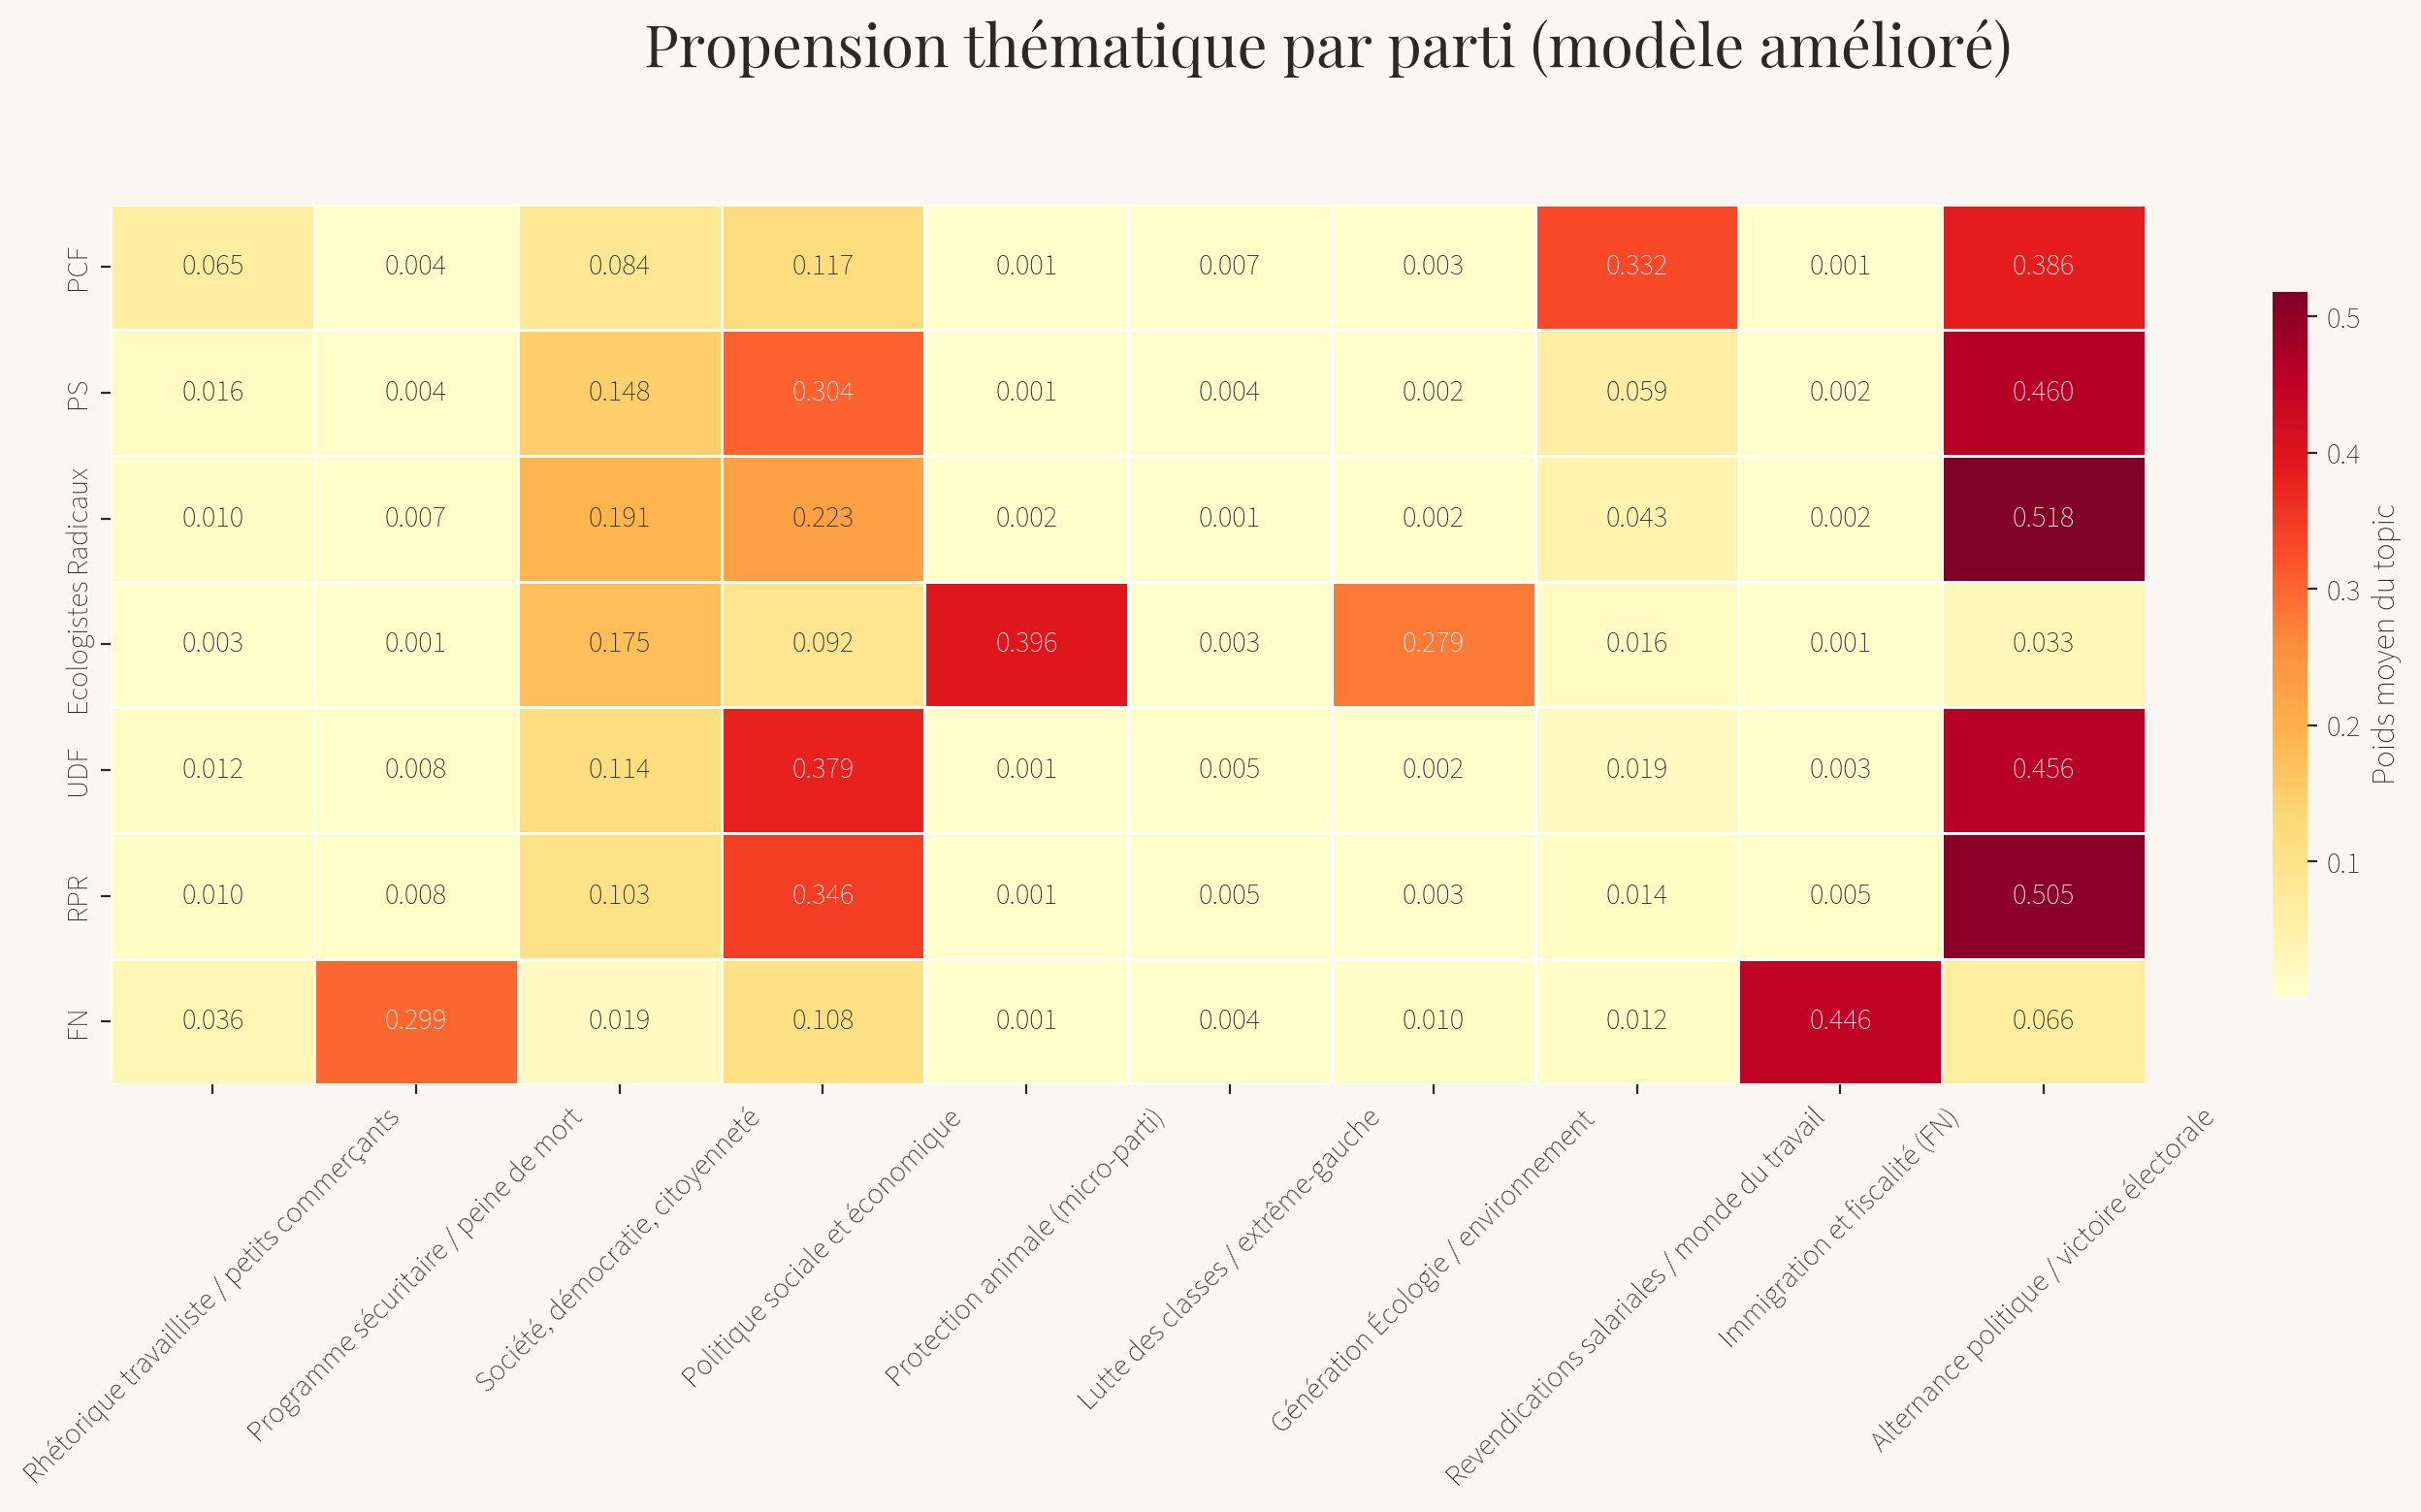
\includegraphics[width=\linewidth]{heatmap_topics_v2_partis.png}
\caption{Full heatmap of topic shares by political family. No topic is exclusive to a single family---the closest is the FN rhetoric topic. Most topics are cross-cutting, reinforcing the claim that differentiation operates through vocabulary, not topic allocation.}
\label{fig:heatmap_full}
\end{figure}

\section{Model comparison and BERTopic}
\label{app:models}

We compared LDA ($k{=}11$, $C_v{=}0.49$, max topic share 23.6\%) with NMF ($k{=}5$, $C_v{=}0.71$, max topic share 84.5\%). NMF's higher coherence is misleading: the model is degenerate, concentrating nearly all documents in one background topic. NMF excels at isolating micro-clusters (animal welfare, specific local issues) but fails as a general decomposition.

We also experimented with BERTopic (Sentence-Transformers + UMAP + HDBSCAN). While it produces semantically coherent clusters, the topics are less stable across seeds, and the dense-embedding framework makes coefficient inspection and log-odds computation impractical. LDA's interpretability---you can read the word lists, inspect the $\theta$ vectors, compute specialisation ratios---was decisive for our research questions.

\section{Methodological notes}
\label{app:method}

\textbf{Reproducibility.} All expensive computations are checkpointed. t-SNE (stochastic) is computed once and saved. LDA uses a fixed random seed.

\textbf{German-language filtering.} Alsace-Moselle departments produce bilingual manifestos. Without filtering, these create a spurious ``German'' topic. We remove them via a language-detection heuristic.

\textbf{OCR quality.} Older documents (1973, 1978) contain more recognition errors: character confusions (\textit{l}/\textit{1}), word splits, header noise. We remove the systematic ``Sciences Po / fonds CEVIPOF'' watermark, but residual noise remains. Post-OCR correction with language models is a natural improvement.

\textbf{Learning curve.} The classifier's performance plateaus at $\sim$60\% of training data, indicating model expressiveness---not data size---is the bottleneck. Fine-tuning CamemBERT would likely improve minority-class performance (Centre, Écologistes).

\end{document}
